\documentclass{article}
\usepackage[utf8]{inputenc}
\usepackage[english]{babel}
\usepackage{setspace}
\usepackage{amssymb}
\usepackage{amsmath}
\usepackage{chngcntr}
\usepackage{float}
\usepackage{tabu}
\usepackage{bm}
\usepackage[lite]{amsrefs}
\usepackage{amsthm}
\usepackage{graphicx}
\usepackage{hyperref}\usepackage{xcolor}
%\graphicspath{ {./img/} }

\usepackage{graphicx}
\graphicspath{ {./images/} }

\usepackage{tikz}
\usetikzlibrary{matrix}

\newcommand{\shrug}[1][]{%
\begin{tikzpicture}[baseline,x=0.8\ht\strutbox,y=0.8\ht\strutbox,line width=0.125ex,#1]
\def\arm{(-2.5,0.95) to (-2,0.95) (-1.9,1) to (-1.5,0) (-1.35,0) to (-0.8,0)};
\draw \arm;
\draw[xscale=-1] \arm;
\def\headpart{(0.6,0) arc[start angle=-40, end angle=40,x radius=0.6,y radius=0.8]};
\draw \headpart;
\draw[xscale=-1] \headpart;
\def\eye{(-0.075,0.15) .. controls (0.02,0) .. (0.075,-0.15)};
\draw[shift={(-0.3,0.8)}] \eye;
\draw[shift={(0,0.85)}] \eye;
% draw mouth
\draw (-0.1,0.2) to [out=15,in=-100] (0.4,0.95); 
\end{tikzpicture}}




\counterwithin*{equation}{section}

\newcommand{\R}{\mathbb{R}}

\makeatletter
\newcommand*\bigcdot{\mathpalette\bigcdot@{1}}
\newcommand*\bigcdot@[2]{\mathbin{\vcenter{\hbox{\scalebox{#2}{$\m@th#1\bullet$}}}}}
\makeatother

\usepackage{afterpage}

\newcommand\blankpage{%
    \null
    \thispagestyle{empty}%
    \addtocounter{page}{-1}%
    \newpage}
    
\newtheorem{theorem}{Theorem}[section]
\newtheorem{definition}[theorem]{Definition}
\newtheorem{observation}[theorem]{Observation}
\newtheorem{corollary}{Corollary}[theorem]
\newtheorem{lemma}[theorem]{Lemma}

%\setlength{\parindent}{0pt}

\DeclareMathOperator*{\argmax}{\arg\!\max}
\DeclareMathOperator*{\argmin}{\arg\!\min}

\newcommand*{\defeq}{\mathrel{\vcenter{\baselineskip0.5ex \lineskiplimit0pt
                     \hbox{\scriptsize.}\hbox{\scriptsize.}}}%
                     =}

\usepackage[]{algorithm2e}


\newcommand*\OR{\ |\ }

\usepackage[top=2.5cm, left=3cm, right=3cm, bottom=4.0cm]{geometry}

\newcommand{\lectureheader}[4]{%
  \begin{minipage}{.3\textwidth}%
    
    \strut\includegraphics[width=\textwidth]{figures/ethlogo.pdf}%
  \end{minipage} \hfill%
  \raisebox{1.5mm}{%
    \begin{minipage}{0.69\textwidth}\sf\flushright%
        \textbf{\Huge #3}\mbox{\hspace{2mm}}\\#4\mbox{\hspace{2mm}}%
    \end{minipage}%
  }\\[-2mm]\hrule%
  \begin{minipage}[t]{0.5\textwidth}\sf\textit{#1} \end{minipage} \hfill%
  \begin{minipage}[t]{0.5\textwidth}\sf\flushright \textit{#2}\end{minipage}%
  \par%
}


\begin{document}

\begin{titlepage} 

\lectureheader{Prof. Ryan Cotterell}
{}
{\Large Natural Language Processing}{Spring 2021}
	\newcommand{\HRule}{\rule{\linewidth}{0.5mm}} 
	
	\center % Centre everything on the page
	{\Huge Course Assignment \# 2}\\
      \quad\newline
	
	{\large\today} \\
	\quad\newline
	%	Author
	%------------------------------------------------
	
	{\Large Andrius Buinovskij \\ \emph{nethz} Username: andriusb \\ Student ID: 18-940-270}\\[0.5cm] 
	\vfill
	
	\vfill\vfill\vfill 
	By submitting this work, I verify that it is my own. That is, I have written my own solutions to each problem for which I am submitting an answer. I have listed above all others with whom I have discussed these answers.
	
	\vfill 
	
\end{titlepage}
\textbf{Q1 a)}

	\begin{align}
		S &\to NP, VP\\
		NP &\to Det, N \OR NP, PP \OR "I" \OR "glasses"\\
		VP &\to VP, PP \OR V, NP\\		
		Det &\to "a" \OR "an"\\
		N &\to "man" \OR "pencil" \OR "ball" \OR "umbrella"\\
		PP &\to P, NP\\
		V &\to "draw" \OR "hit"\\
		P &\to "with" 
	\end{align}
	
\textbf{Q1 b)}

	Warning: advanced calculations ahead (instead of probabilities We just do counts first):

	\begin{align}
		S &\to NP, VP (4)\\
		NP (14) &\to Det, N (7) \OR NP, PP (2)\OR "I" (4)\OR "glasses" (1)\\
		VP (6)&\to VP, PP (2)\OR V, NP (4)\\		
		Det (7)&\to "a" (6) \OR "an"(1)\\
		N (7)&\to "man" (4)\OR "pencil"(1) \OR "ball"(1) \OR "umbrella"(1)\\
		PP (4)&\to P, NP (4)\\
		V (4)&\to "draw" (2) \OR "hit"(2)\\
		P (4)&\to "with" (4) 
	\end{align}
	
	Convert to probabilities (rounded, for precise figures just divide counts on the right by total counts on the left):
	
	\begin{align}
		S &\to NP, VP (1.0)\\
		NP  &\to Det, N (0.5) \OR NP, PP (0.14)\OR "I" (0.29)\OR "glasses" (0.7)\\
		VP (&\to VP, PP (2=0.33)\OR V, NP (0.66)\\		
		Det &\to "a" (0.86( \OR "an"(0.14)\\
		N &\to "man" (0.57)\OR "pencil"(0.14) \OR "ball"(0.14) \OR "umbrella"(0.14)\\
		PP &\to P, NP (1)\\
		V &\to "draw" (0.5) \OR "hit"(0.5)\\
		P &\to "with" (1) 
	\end{align}
	
\textbf{Q1 c)}

	Our goal is to have different likelihood of expansions on noun phrase depending on whether the expansion is going to be an object or a subject.

	I suppose a logical way of going about it would be to replace the noun phrase non-terminal with two other non terminals - object phrase ($OP$) and subject phrase ($SP$). 
	
	\begin{align}
		S &\to NP, VP (1.0)\\
		NP &\to SP \OR  OP\\
		SP &\to Det, N (0.5) \OR NP, PP (0.14)\OR "I" (0.29)\OR "glasses" (0.7)\\
		OP &\to Det, N (0.5) \OR NP, PP (0.14)\OR "I" (0.29)\OR "glasses" (0.7)\\
		VP (&\to VP, PP (2=0.33)\OR V, NP (0.66)\\		
		Det &\to "a" (0.86( \OR "an"(0.14)\\
		N &\to "man" (0.57)\OR "pencil"(0.14) \OR "ball"(0.14) \OR "umbrella"(0.14)\\
		PP &\to P, NP (1)\\
		V &\to "draw" (0.5) \OR "hit"(0.5)\\
		P &\to "with" (1) 
	\end{align}
	
	Here are the counts as before:
	
	\begin{align}
		S &\to NP, VP (1.0)\\
		NP (14)&\to SP (4)\OR  OP (10)\\
		SP (4) &\to Det, N (0) \OR NP, PP (0)\OR "I" (4) \OR "glasses" (0)\\
		OP (10)&\to  Det, N (7) \OR NP, PP (2)\OR "I" (0)\OR "glasses" (1)\\
		VP (&\to VP, PP (2=0.33)\OR V, NP (0.66)\\		
		Det &\to "a" (0.86( \OR "an"(0.14)\\
		N &\to "man" (0.57)\OR "pencil"(0.14) \OR "ball"(0.14) \OR "umbrella"(0.14)\\
		PP &\to P, NP (1)\\
		V &\to "draw" (0.5) \OR "hit"(0.5)\\
		P &\to "with" (1) 
	\end{align}
	
	Finally converting to probabilities:
	
	\begin{align}
		S &\to NP, VP (1.0)\\
		NP &\to SP (0.29)\OR  OP (0.71)\\
		SP (4) &\to Det, N (0) \OR NP, PP (0)\OR "I" (1) \OR "glasses" (0)\\
		OP (10)&\to  Det, N (0.7) \OR NP, PP (0.2)\OR "I" (0)\OR "glasses" (0.1)\\
		VP (&\to VP, PP (2=0.33)\OR V, NP (0.66)\\		
		Det &\to "a" (0.86( \OR "an"(0.14)\\
		N &\to "man" (0.57)\OR "pencil"(0.14) \OR "ball"(0.14) \OR "umbrella"(0.14)\\
		PP &\to P, NP (1)\\
		V &\to "draw" (0.5) \OR "hit"(0.5)\\
		P &\to "with" (1) 
	\end{align}
	
	Well this at least shows that subject phrases are likely to be "I", and object phrases are unlikely to be "I", so it's capturing some of what We wanted to. 
	
	There is a problem here of course - nothing is stopping anyone from using $SP$ instead of $OP$ wherever they like, so the onus is on the user of the grammar to use the subject non-terminal for subjects and the object non-terminal for objects.
	
\textbf{Q1 d)}
	
	\begin{align}
		S &\to NP, VP^+\\
		NP &\to Det, N^+ \OR NP^+, PP \OR "I" \OR "glasses"\\
		VP &\to VP^+, PP \OR V^+, NP\\		
		Det &\to "a" \OR "an"\\
		N &\to "man" \OR "pencil" \OR "ball" \OR "umbrella"\\
		PP &\to P, NP^+\\
		V &\to "draw" \OR "hit"\\
		P &\to "with" 
	\end{align}
	
	\includegraphics[angle=90,origin=c,width=\textwidth]{figures/headed_parse_tree}
	
	
	
\textbf{Q2 a)}

	So, it is my understanding that for the projective dependency tree, to obtain the score We would simply take all dependency pairs and multiply the scores corresponding to those dependencies (taking care to pay attention to the direction of the dependency etc.)
	
	To obtain the score of a lexicalized probabilistic context free grammar tree, one also simply multiplies the score for each "rule" applied, except this rule is also lexicalized so You have very many parameters indeed (page 15 from \href{http://www.cs.columbia.edu/~mcollins/courses/nlp2011/notes/lexpcfgs.pdf}{\_ click me\_}.)
	
	With all that out of the way, I would construct a weighted lexicalized CFG as follows: 
	
	1. Add root productions $R \to X_j$, $j\in 1\ldots M$.
	
	2. Add self-productions $X_j \to j$.
	
	3. For each production $\psi(i\to j)$, add bidirectional productions to the language as follows:
	
	\begin{align}
		X_i \to X_i^+, X_j\\
		X_i \to X_j, X_i^+
	\end{align}
	
	And of course they weight for that transformation corresponds to the value of $\psi(i\to j)$ does not You anything about the ordering of words within a sentence.
	
	The reason for adding bidirectional rules is that just having access to the set of weights generated by 
	
	And that's all She wrote.
	
\textbf{Q2 b)}

	So the dependency tree would simply be $ROOT\to fish$, $fish\to they$, and the score would be $\psi(ROOT, fish)\cdot \psi(fish, they)$.
	
	In our CFG We would end up with $ROOT\to S$, then $S\to NP$, 
	
	\includegraphics[angle=90,origin=c,width=\textwidth]{figures/relational_parse}
	

	
\newpage
\textbf{Q4 a)}

	\begin{table}[ht]
        \centering
        \fontsize{10}{10}\selectfont
        \renewcommand{\arraystretch}{1.2} % vertical padding
        \setlength{\tabcolsep}{0.5em} % for the horizontal padding
        \begin{tabular}{l|l|l|l}
        \textbf{number} & \textbf{sample strings} & \textbf{accepted} & \textbf{weight} \\ \hline
        1 & educational is this not & NO &  \\
        2 & is this assignment educational & NO & \\
        3 & not educational is not educational  & YES & 12 \\
        4 & this assignment is not educational & YES & 7 \\
        5 & is this assignment educational & NO &  \\
        6 & this assignment course is educational & NO  &  \\
        7 & is this assignment not educational &  YES & 15 \\
        8 & this assignment not & YES & 8 \\
        9 & this course assignment is not educational & YES  & 12 \\
        10 & this course is not not educational & YES & 21 \\
        11 & not educational is this & YES & 10 \\
        12 & course assignment is not educational & YES & 10 \\
        13 & not this assignment is educational & NO &  \\
        14 & not not not educational & YES & 25 \\
        15 & is this course assignment not educational  & YES & 18 \\
        16 & course assignment is this & YES & 8 \\
        17 & this course is interesting & NO &  \\
        18 & this course assignment not educational & YES & 14
        \end{tabular}
        \caption{Some strings from $\mathcal{Y}_{\geq 2, \leq 6}$}
        \label{tab:wfst_strings}
        \end{table}
	
	
\textbf{Q4 b)}

	Cost matrices on left, backtracking matrices on the right.
	
	"inf" means an infinite cost, i.e. no path exists, and similarly "N" in the backtracking matrix means a backtrack is not possible.
	
Iteration 0

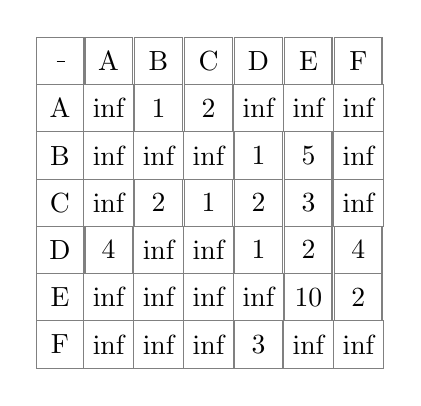
\begin{tikzpicture}
\matrix[matrix of nodes,nodes={draw=gray, anchor=center, minimum size=.6cm}, column sep=-\pgflinewidth, row sep=-\pgflinewidth] (A) {
 &\_ & A & B & C & D & E & F \\ & A & inf & 1 & 2 & inf & inf & inf\\
 & B & inf & inf & inf & 1 & 5 & inf\\
 & C & inf & 2 & 1 & 2 & 3 & inf\\
 & D & 4 & inf & inf & 1 & 2 & 4\\
 & E & inf & inf & inf & inf & 10 & 2\\
 & F & inf & inf & inf & 3 & inf & inf\\
};
\end{tikzpicture}
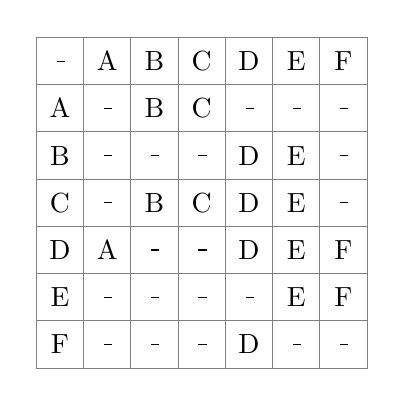
\begin{tikzpicture}
\matrix[matrix of nodes,nodes={draw=gray, anchor=center, minimum size=.6cm}, column sep=-\pgflinewidth, row sep=-\pgflinewidth] (A) {
 &\_ & A & B & C & D & E & F \\ & A & \_ & B & C & \_ & \_ & \_\\
 & B & \_ & \_ & \_ & D & E & \_\\
 & C & \_ & B & C & D & E & \_\\
 & D & A & \_ & \_ & D & E & F\\
 & E & \_ & \_ & \_ & \_ & E & F\\
 & F & \_ & \_ & \_ & D & \_ & \_\\
};
\end{tikzpicture}


Iteration 1

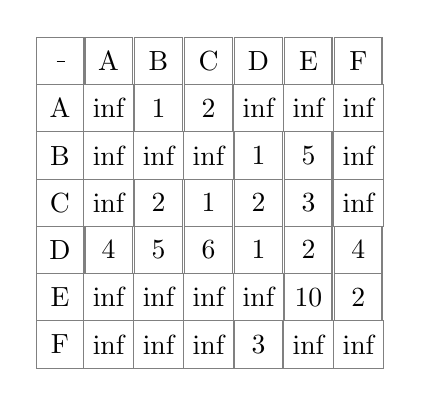
\begin{tikzpicture}
\matrix[matrix of nodes,nodes={draw=gray, anchor=center, minimum size=.6cm}, column sep=-\pgflinewidth, row sep=-\pgflinewidth] (A) {
 &\_ & A & B & C & D & E & F \\ & A & inf & 1 & 2 & inf & inf & inf\\
 & B & inf & inf & inf & 1 & 5 & inf\\
 & C & inf & 2 & 1 & 2 & 3 & inf\\
 & D & 4 & 5 & 6 & 1 & 2 & 4\\
 & E & inf & inf & inf & inf & 10 & 2\\
 & F & inf & inf & inf & 3 & inf & inf\\
};
\end{tikzpicture}
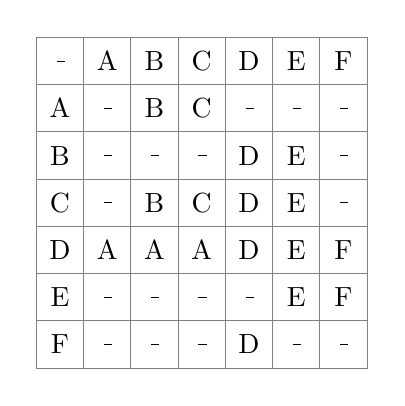
\begin{tikzpicture}
\matrix[matrix of nodes,nodes={draw=gray, anchor=center, minimum size=.6cm}, column sep=-\pgflinewidth, row sep=-\pgflinewidth] (A) {
 &\_ & A & B & C & D & E & F \\ & A & \_ & B & C & \_ & \_ & \_\\
 & B & \_ & \_ & \_ & D & E & \_\\
 & C & \_ & B & C & D & E & \_\\
 & D & A & A & A & D & E & F\\
 & E & \_ & \_ & \_ & \_ & E & F\\
 & F & \_ & \_ & \_ & D & \_ & \_\\
};
\end{tikzpicture}


Iteration 2

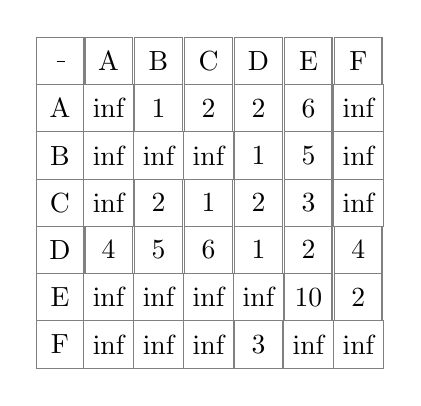
\begin{tikzpicture}
\matrix[matrix of nodes,nodes={draw=gray, anchor=center, minimum size=.6cm}, column sep=-\pgflinewidth, row sep=-\pgflinewidth] (A) {
 &\_ & A & B & C & D & E & F \\ & A & inf & 1 & 2 & 2 & 6 & inf\\
 & B & inf & inf & inf & 1 & 5 & inf\\
 & C & inf & 2 & 1 & 2 & 3 & inf\\
 & D & 4 & 5 & 6 & 1 & 2 & 4\\
 & E & inf & inf & inf & inf & 10 & 2\\
 & F & inf & inf & inf & 3 & inf & inf\\
};
\end{tikzpicture}
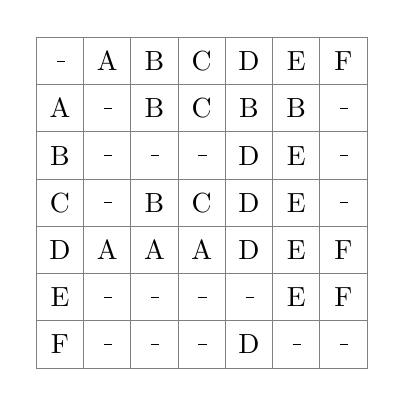
\begin{tikzpicture}
\matrix[matrix of nodes,nodes={draw=gray, anchor=center, minimum size=.6cm}, column sep=-\pgflinewidth, row sep=-\pgflinewidth] (A) {
 &\_ & A & B & C & D & E & F \\ & A & \_ & B & C & B & B & \_\\
 & B & \_ & \_ & \_ & D & E & \_\\
 & C & \_ & B & C & D & E & \_\\
 & D & A & A & A & D & E & F\\
 & E & \_ & \_ & \_ & \_ & E & F\\
 & F & \_ & \_ & \_ & D & \_ & \_\\
};
\end{tikzpicture}


Iteration 3

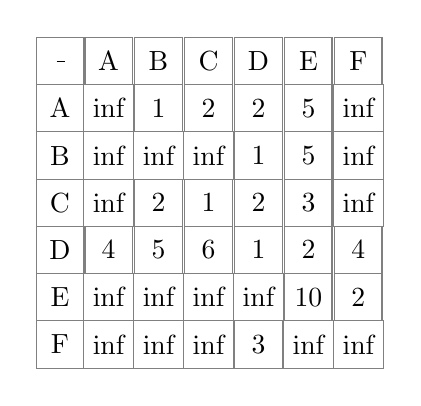
\begin{tikzpicture}
\matrix[matrix of nodes,nodes={draw=gray, anchor=center, minimum size=.6cm}, column sep=-\pgflinewidth, row sep=-\pgflinewidth] (A) {
 &\_ & A & B & C & D & E & F \\ & A & inf & 1 & 2 & 2 & 5 & inf\\
 & B & inf & inf & inf & 1 & 5 & inf\\
 & C & inf & 2 & 1 & 2 & 3 & inf\\
 & D & 4 & 5 & 6 & 1 & 2 & 4\\
 & E & inf & inf & inf & inf & 10 & 2\\
 & F & inf & inf & inf & 3 & inf & inf\\
};
\end{tikzpicture}
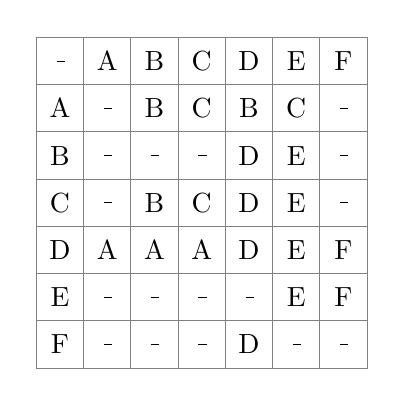
\begin{tikzpicture}
\matrix[matrix of nodes,nodes={draw=gray, anchor=center, minimum size=.6cm}, column sep=-\pgflinewidth, row sep=-\pgflinewidth] (A) {
 &\_ & A & B & C & D & E & F \\ & A & \_ & B & C & B & C & \_\\
 & B & \_ & \_ & \_ & D & E & \_\\
 & C & \_ & B & C & D & E & \_\\
 & D & A & A & A & D & E & F\\
 & E & \_ & \_ & \_ & \_ & E & F\\
 & F & \_ & \_ & \_ & D & \_ & \_\\
};
\end{tikzpicture}


Iteration 4

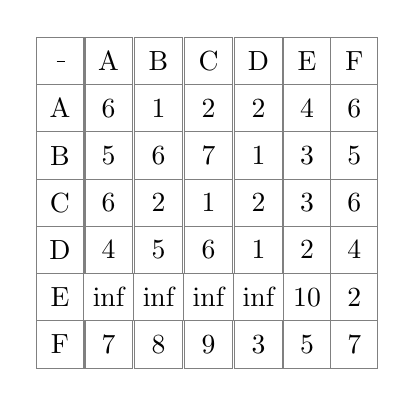
\begin{tikzpicture}
\matrix[matrix of nodes,nodes={draw=gray, anchor=center, minimum size=.6cm}, column sep=-\pgflinewidth, row sep=-\pgflinewidth] (A) {
 &\_ & A & B & C & D & E & F \\ & A & 6 & 1 & 2 & 2 & 4 & 6\\
 & B & 5 & 6 & 7 & 1 & 3 & 5\\
 & C & 6 & 2 & 1 & 2 & 3 & 6\\
 & D & 4 & 5 & 6 & 1 & 2 & 4\\
 & E & inf & inf & inf & inf & 10 & 2\\
 & F & 7 & 8 & 9 & 3 & 5 & 7\\
};
\end{tikzpicture}
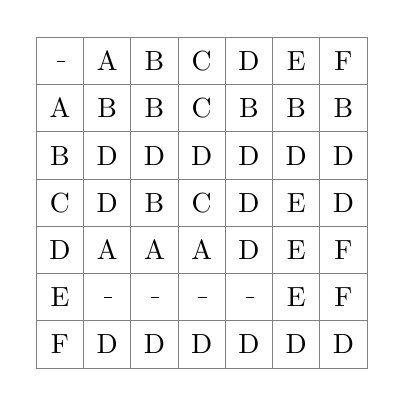
\begin{tikzpicture}
\matrix[matrix of nodes,nodes={draw=gray, anchor=center, minimum size=.6cm}, column sep=-\pgflinewidth, row sep=-\pgflinewidth] (A) {
 &\_ & A & B & C & D & E & F \\ & A & B & B & C & B & B & B\\
 & B & D & D & D & D & D & D\\
 & C & D & B & C & D & E & D\\
 & D & A & A & A & D & E & F\\
 & E & \_ & \_ & \_ & \_ & E & F\\
 & F & D & D & D & D & D & D\\
};
\end{tikzpicture}


Iteration 5

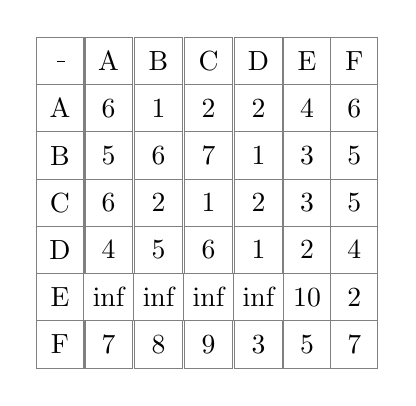
\begin{tikzpicture}
\matrix[matrix of nodes,nodes={draw=gray, anchor=center, minimum size=.6cm}, column sep=-\pgflinewidth, row sep=-\pgflinewidth] (A) {
 &\_ & A & B & C & D & E & F \\ & A & 6 & 1 & 2 & 2 & 4 & 6\\
 & B & 5 & 6 & 7 & 1 & 3 & 5\\
 & C & 6 & 2 & 1 & 2 & 3 & 5\\
 & D & 4 & 5 & 6 & 1 & 2 & 4\\
 & E & inf & inf & inf & inf & 10 & 2\\
 & F & 7 & 8 & 9 & 3 & 5 & 7\\
};
\end{tikzpicture}
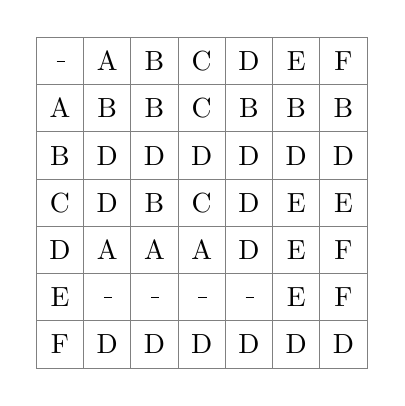
\begin{tikzpicture}
\matrix[matrix of nodes,nodes={draw=gray, anchor=center, minimum size=.6cm}, column sep=-\pgflinewidth, row sep=-\pgflinewidth] (A) {
 &\_ & A & B & C & D & E & F \\ & A & B & B & C & B & B & B\\
 & B & D & D & D & D & D & D\\
 & C & D & B & C & D & E & E\\
 & D & A & A & A & D & E & F\\
 & E & \_ & \_ & \_ & \_ & E & F\\
 & F & D & D & D & D & D & D\\
};
\end{tikzpicture}

Final 6th iteration

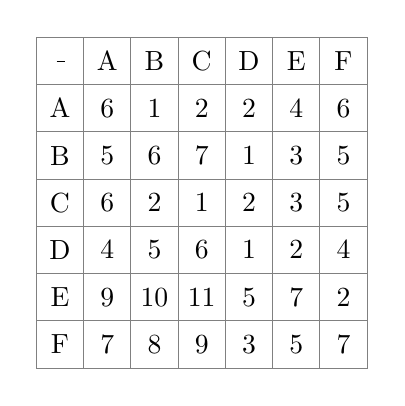
\begin{tikzpicture}
\matrix[matrix of nodes,nodes={draw=gray, anchor=center, minimum size=.6cm}, column sep=-\pgflinewidth, row sep=-\pgflinewidth] (A) {
 &\_ & A & B & C & D & E & F \\ & A & 6 & 1 & 2 & 2 & 4 & 6\\
 & B & 5 & 6 & 7 & 1 & 3 & 5\\
 & C & 6 & 2 & 1 & 2 & 3 & 5\\
 & D & 4 & 5 & 6 & 1 & 2 & 4\\
 & E & 9 & 10 & 11 & 5 & 7 & 2\\
 & F & 7 & 8 & 9 & 3 & 5 & 7\\
};
\end{tikzpicture}
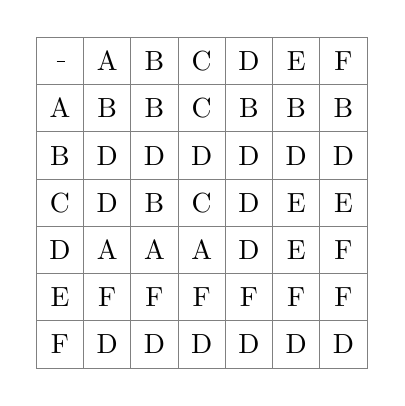
\begin{tikzpicture}
\matrix[matrix of nodes,nodes={draw=gray, anchor=center, minimum size=.6cm}, column sep=-\pgflinewidth, row sep=-\pgflinewidth] (A) {
 &\_ & A & B & C & D & E & F \\ & A & B & B & C & B & B & B\\
 & B & D & D & D & D & D & D\\
 & C & D & B & C & D & E & E\\
 & D & A & A & A & D & E & F\\
 & E & F & F & F & F & F & F\\
 & F & D & D & D & D & D & D\\
};
\end{tikzpicture}
	
\textbf{Q4 c)}

	The number of iterations is bound by $\mathcal{O}(N^3)$, where $N$ is the number of nodes. 
	
	The algorithm terminated after 6 iterations, so after looking at all of the nodes.
	
\textbf{Q4 d)}
	
	The time complexity is $\mathcal{O}(N^3)$ and for the method I used the space complexity is $N^2$. Strictly speaking it's more like $4N^2$ since I was keeping new and old versions of matrices around in my implementation, but this can be reduced. Asymptotically, it's simply $\mathcal{O}(N^2)$ for space complexity and $\mathcal{O}(N^3)$ for time complexity.
	
	Backtracking takes $\mathcal{O}(n)$ and is achieved as follows: let starting node be $u$ and ending node be $v$. Now take the $v$'th column of the backtracking matrix, and begin at the $u$'th entry. The value of the $u$'th entry is the next node in the shortest path. Then simply follow the entries until the desired destination is reached. 
	
	This makes sense intuitively - it may be the case that to go from $u$ to $v$ one has to traverse all the nodes, but no node should be traversed more than once since if it were, then there is a cycle in the path that could be cut out.
	
\end{document} 